\chapter{Hardware Implementation}

\section{Project Hierarchy}
Programming the FPGA to communicate with the HPS is no trivial task.
Luckily, there exists a golden system reference design~\cite{Rocket1} for the board in use for this project.
Unfortunately, support for certain versions of Quartus are missing from the GSRD download database, including the version used for this project, 16.0.
While the design can be opened with a different version of the software, it causes a series of conflicts usually related to using IP cores that have changed over the iterations.
To circumvent this issue cleanly, GSRD version 14.1 was downloaded and compiled on a separate install of Quartus II 14.1.
This allowed the reference design to be studied in detail, and the sections required for this project to be rebuilt with Quartus Prime 16.0.

\begin{figure}[H]
  \centering
  \begin{forest}
  for tree={
    align=center,
    font=\ttfamily,
    edge+={thick, -{Stealth[]}},
    l sep'+=10pt,
    fork sep'=10pt,
  },
  forked edges,
  if level=0{
    inner xsep=0pt,
    tikz={\draw [thick] (.children first) -- (.children last);}
  }{},
  [sys\_top
    [reset]
    [debounce]
    [soc\_system
      [hps]
      [hps\_only\_master]
      [jtag\_uart]
      [button\_pio]
      [...]
    ]
    [edge\_detector]
    [...]
  ]
\end{forest}
  \caption{Hierarchy of the Golden Reference Design}
  \label{Golden Hierarchy}
\end{figure}

By examining the structure of the reference design, we see that it has a top-level wrapper called the \texttt{sys\_top}, which instantiates the Qsys system \texttt{soc\_system} and a few IP blocks that handles the low level hardware controls on the development board.
This Qsys system is of the most interest to us as it contains the module \texttt{hps}.
In \texttt{hps}, there are 3 ports named \texttt{h2f\_axi\_master}, \texttt{h2f\_axi\_slave}, and \texttt{h2f\_lw\_axi\_master}, cooresponding to the bridges exposed by the HPS for connections~\cite{Altera6}.

With this knowledge, we can insert the testbench design into this hierarchy by having it wrapped into a Qsys module, with an open port that works as a slave to the AXI bridge.
As the traffic passing through the HPS-FPGA bridge is minimal in our design, the lightweight bridge will be used for its simplicity.

As the testbench only requires a list of registers to be sparingly read and written to, the logic required for the signals on the Avalon slave interface can be handwritten according to the interface specifications~\cite{Intel3} without much trouble.

By following the naming conventions  the signals allows Qsys Component Editor to automatically detect the Avalon slave from this module at analysis.
This saves the troubles of editing the \texttt{\_hw.tcl} file.
This is done in the module \texttt{text\_wrapper}.

Since Qsys is chosen as the user interface, it makes sense to also put the DUT and the reference design at this level in the hierarchy.
This means that the user only needs to use Qsys to swap in new designs.
As such, other than handling the interface to the HPS, the wrapper module also exposes conduits that connects to the DUT and the references designs.

In addition, the PLL and its reconfiguration module are also instantiated at this level since as packaged IP cores, Qsys is designed for such integrations.

\begin{figure}[H]
  \centering
  \begin{forest}
  for tree={
    align=center,
    font=\ttfamily,
    edge+={thick},
    l sep'+=10pt,
    fork sep'=10pt,
  },
  forked edges,
  if level=0{
    inner xsep=0pt,
    tikz={\draw [thick] (.children first) -- (.children last);}
  }{},
  [\textbf{sys\_top}
    [reset]
    [debounce]
    [\textbf{soc\_system}
      [\textbf{hps}]
      [\textbf{pll}]
      [\textbf{pll\_reconfig}]
      [\textbf{test\_wrapper}
        [\textbf{testbench}
          [randomiser]
          [driver]
          [monitor
            [sub\_mon]
          ]
          [scoreboard]
        ]
      ]
      [\textbf{dut}]
      [\textbf{ref}]
      [...]
    ]
    [edge\_detector]
    [...]
  ]
\end{forest}
  \caption{Hierarchy of the Full Hardware System}
  \label{Hierarchy}
\end{figure}

The main section of the testbench is instantiated in the wrapper as a separate module aptly named \texttt{testbench}.
This module instantiates and connects all main components of the testbench.
While this module seems unnecessary, being another wrapper in a bigger wrapper, it does however, provide 2 advantages.

Firstly, it simplifies the development cycle of the framework.
During the compilation of a Qsys system, all relevant files are copied into a folder and the system is rendered as a Verilog file that has its direct dependencies contained in that folder.
While this is arguably a benefit in terms of dependency management, it makes the development more difficult since whenever something is changed in the interface between testbench modules, the entire \texttt{soc\_system} needs to be recompiled to update the dependencies.
If forgotten, it can cause confusions as the testbench could be still on the old iteration even though a new compilation at the \texttt{sys\_top} level has been performed.

Secondly, it makes the simulation of the testbench more straight forward.
Verifying the correctness of the Avalon slave in the wrapper is important, but there is no need to go through the interface protocol whenever a new input signal is desired in testbench simulations.
Having the \texttt{testbench} module allows direct manipulation and examination of the signals in and out of the testbench, without worrying about the HPS side of things in simulations.

\section{Randomiser}

\begin{figure}[H]
  \centering
  \begin{tikzpicture}
  [
    x=1em, y=1em,
    block/.style =
      {draw, rectangle, align=center, minimum width=4em, minimum height=6em},
    iarrow/.style =
      {<-, >={Stealth}, font=\ttfamily},
    oarrow/.style =
      {->, >={Stealth}, font=\ttfamily}
  ]

\node[block, label=above:Randomiser] (r) at (0,0) {};

\draw [iarrow] ($(r.west)+(0,2)$) -- ++(left:3) node[left] {clk};
\draw [iarrow] ($(r.west)+(0,1)$) -- ++(left:3) node[left] {reset};
\draw [iarrow] ($(r.west)-(0,1)$) -- ++(left:3) node[left] {enable};
\draw [iarrow] ($(r.west)-(0,2)$) -- ++(left:3) node[left] {initial};

\draw [oarrow] ($(r.east)+(0,2)$) -- ++(right:3) node[right] {out};

\end{tikzpicture}
  \caption{Randomiser Block Diagram}
  \label{RandomiserBlk}
\end{figure}

Implementing the randomiser is straight forward.
A possible set of taps for a 32-bit Galois LFSR is [32, 30, 26, 25].
Referring back at Figure~\ref{GalLFSR} on page~\pageref{GalLFSR},
the logic is to XOR the bits left of the taps with bit 0, and simple right shift for all other bits.
For driver to control the randomiser, an enable signal and an initial signal is added as input in addition to clock and reset.
The initial signal seeds the LFSR.

\section{Driver}

\begin{figure}[H]
  \centering
  \begin{tikzpicture}
  [
    x=1em, y=1em,
    block/.style =
      {draw, rectangle, align=center, minimum width=4em, minimum height=10em},
    sarrow/.style =
      {>={Stealth}, font=\ttfamily},
    darrow/.style =
      {double distance=1.5pt, >={Stealth}, font=\ttfamily}
  ]

\node[block, label=above:Driver] (r) at (0,0) {};

\draw [<-, sarrow] ($(r.west)+(0,4.5)$) -- ++(left:3) node[left] {clk};
\draw [<-, sarrow] ($(r.west)+(0,3.5)$) -- ++(left:3) node[left] {reset};

\draw [<-, sarrow] ($(r.west)+(0,1.5)$) -- ++(left:3) node[left] {f\_select};
\draw [<-, darrow] ($(r.west)+(0,0.5)$) -- ++(left:3) node[left] {f\_manual};
\draw [<-, sarrow] ($(r.west)-(0,0.5)$) -- ++(left:3) node[left] {f\_bitset};
\draw [<-, sarrow] ($(r.west)-(0,1.5)$) -- ++(left:3) node[left] {f\_bitclr};
\draw [<-, darrow] ($(r.west)-(0,2.5)$) -- ++(left:3) node[left] {rand\_*};

\draw [<-, darrow] ($(r.west)-(0,4.5)$) -- ++(left:3) node[left] {dut\_out};

\draw [->, sarrow] ($(r.east)-(0,4.5)$) -- ++(right:3) node[right] {dut\_delay};

\draw [->, darrow] ($(r.east)-(0,1.5)$) -- ++(right:3) node[right] {drive\_*};
\draw [->, darrow] ($(r.east)-(0,2.5)$) -- ++(right:3) node[right] {drive\_delayed\_*};
\end{tikzpicture}
  \caption{Driver Block Diagram}
  \label{DriverBlk}
\end{figure}

The filter select signal \texttt{f\_select} selects the mode of operation of the driver.
When it is set, the driver will read from \texttt{f\_manual} and feed them to the output.
Otherwise, the driver will take the output of the randomisers at \texttt{rand\_*}, set and clearing specific bits according to \texttt{f\_bitset} and \texttt{f\_bitclr}.

The output is immediately sent to the DUT from the ports \texttt{drive\_*}.
The output is also delayed for a number of cycles before being sent to the monitor from the ports \texttt{drive\_delayed\_*}.
This delay is known and thus can be configured by the user before compiling the testbench.

\subsection{Delay Tester}

Since finding out the delay of the DUT is useful for further simplifying the configuration process of the framework, a delay tester is built within the driver.
It counts the number of cycles for the DUT to produce its output as \texttt{dut\_delay}, but it still has a few limitations in its design.
As such, using this to reconfigure the driver to monitor delay on the fly is not yet possible.
How this might be achieved will be discussed in the Future Work chapter of this report.

The delay tester is built with a simple FSM.

\begin{figure}[H]
  \centering
  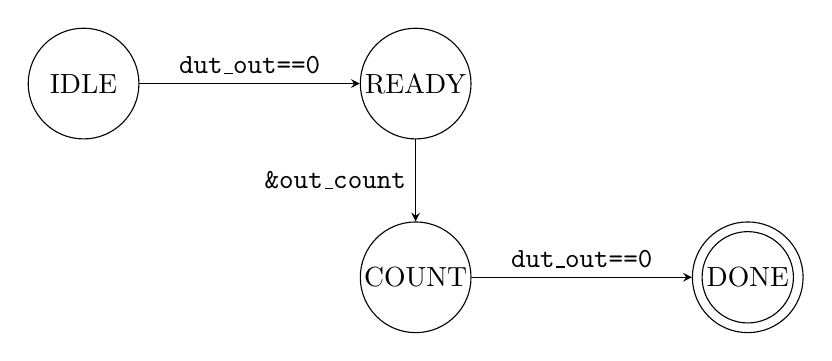
\begin{tikzpicture}
  [
    x=1em, y=1em,
    node/.style =
      {draw, circle, align=center, inner sep=0pt, minimum size=4em},
    sarrow/.style =
      { ->, >=stealth, font=\ttfamily}
  ]
  \node [node] at ( 0, 7)  (i) {IDLE};
  \node [node] at (12, 7) (r) {READY};
  \node [node] at (12, 0)  (c) {COUNT};
  \node [node] at (24, 0)  (d) {DONE};
  \node [draw, circle, inner sep=0pt, minimum size=3.3em] at (24, 0)  (dd) {};

  \draw [sarrow] (i.east)  -- node[above] {dut\_out==0}  (r.west);
  \draw [sarrow] (r.south) -- node[left]  {\&out\_count} (c.north);
  \draw [sarrow] (c.east)  -- node[above] {dut\_out==0}  (d.west);
\end{tikzpicture}
  \caption{Delay Tester FSM}
  \label{DelayTesterFSM}
\end{figure}

We first start a counter called \texttt{out\_count}.
Whenever this reaches all 1's, the driver output is set to some value with a known safe DUT output.
In this example, the safe output value is 0, which means when the delay tester is active, no other output from the driver can result in a DUT output of 0.

\begin{figure}[H]
  \centering
  \input{illu/delay_tester}
  \caption{3-bit Delay Tester Waveform}
  \label{DelayTesterWF}
\end{figure}

The FSM starts in state IDLE.
When the first 0 output is detected from the DUT, the FSM enters the READY state.
It now knows that it can enter the COUNT state when the \texttt{out\_count} becomes all 1's again, triggering the next safe test input.
The FSM leaves the COUNT state for the DONE state when the safe output of 0 is detected.
The delay tester process is now complete and \texttt{out\_count} can be deactivated.

With this, the DUT's delay in clock cycles is the same as the number of cycles that the FSM stayed in state COUNT.
The delay counter \texttt{delay\_out} increments itself every cycle if the FSM is in that state.
When the FSM enters the DONE state, we the value of the delay counter is the delay of the DUT.
With a 3-bit counter as shown in the timing diagram, it can measure this delay for up to 8 clock cycles.
Longer delays can be measured by extending the width of \texttt{out\_count}.

\section{Monitor}



\subsection{Sub Monitors}

\begin{figure}[H]
  \centering
  \begin{tikztimingtable}
    [
      xscale=4,
      timing/d/background/.style={fill=white},
      timing/font=\ttfamily
    ]
    dist\_ctr & D{8} 2{D{1}D{2}D{4}D{8}} D{1}D{2}         \\
    a & U D{AA}D{AB}D{AC}D{AD}D{AE}D{AF}D{AG}D{AH}D{AI} U \\
    b & U D{BA}D{BB}D{BC}D{BD}D{BE}D{BF}D{BG}D{BH}D{BI} U \\
    s & 3U D{SA}D{SB}D{SC}D{SD}D{[red]SK}D{SF}D{SG}D      \\
    \\
    dist\_ctr  [0] & L 2{H 3L} HL \\
    a\_mon     [0] & U 4D{AA} 4D{AE} 2D{AI} \\
    b\_mon     [0] & U 4D{BA} 4D{BE} 2D{BI} \\
    s\_mon     [0] & 2U 4D{SA} 4D{SE} D \\
    sub\_event [0] & 8LH2L \\
  \extracode
    % Add vertical lines in two colors
    \begin{pgfonlayer}{background}
      \begin{scope}[semitransparent,semithick]
        \vertlines{1,2,...,10}
      \end{scope}
    \end{pgfonlayer}
  \end{tikztimingtable}
  \caption{Distributed Monitoring System}
  \label{DisMon}
\end{figure}

\section{Scoreboard}


